%	Größen in TeX:
%		mm, cm, ... uninteressant
%		1 em = Schriftgröße, ursprünglich
%		1 ex = Schriftgröße, skaliert auf die Box in welcher sich die Schrift befindet
%		1 pt = ein Pixel nur kann man nicht von echten Pixeln wie auf einem Bildschirm sprechen
%		\textwidth, \paperwidth, ...

\documentclass[11pt,toc,multi=tcblisting]{article}
\renewcommand{\familydefault}{\sfdefault}
\setcounter{secnumdepth}{6}

\usepackage[left=2cm,right=2cm]{geometry}
%\usepackage[document]{ragged2e} % Damit alles: Links aligned (der linkeste Punkt eines jeden Buchstaben ist auf einer Linie für alle zeilen) und so viel Platz nach rechts ausnutzt, wie möglich (nein, macht TeX nicht standardmäßig); muss man nicht für das gesamte Dokument machen (wie hier), geht auch per \raggedright oder \RaggedRight für/vor Paragraphen; gibt auch Umgebungen für rechtsbündigen Text https://de.overleaf.com/learn/latex/Text_alignment
\usepackage[dvipsnames]{xcolor}
\usepackage{booktabs,array}
\usepackage[author={Hendrik Theede}]{pdfcomment}
\usepackage{tabularx}


\usepackage[utf8]{inputenc}
\usepackage[T1]{fontenc}

\usepackage{inconsolata}
\usepackage[htt]{hyphenat}
\usepackage{listings}
% Note: lstset does not allow unnecessary linebreaks
\lstdefinestyle{texstyle}{
	% Colors
	backgroundcolor=\color{white},
    commentstyle=\color{SeaGreen},
    keywordstyle=\color{Magenta},
    numberstyle=\tiny\color{red},
    stringstyle=\color{Fuchsia},
    basicstyle=\ttfamily\footnotesize\color{black},
	% Linebreaks and Whitespace
    breaklines=true,% Sagt: Bei benötigtem Zeilenumbruch gehen wir in eine neue Zeile
	%breakatwhitespace=true,   
	showspaces=false,                
    showstringspaces=false,
    showtabs=false,
	frame=single,
	xleftmargin=13pt,
	aboveskip=13pt,
	%
	% Indentation
	tabsize=2,
	breakindent=13pt,
    framesep=2mm,
    framerule=0mm,
    abovecaptionskip=5mm,
    aboveskip=\baselineskip,
    belowskip=\baselineskip,
	lineskip=1ex,
	postbreak=\raisebox{0ex}[0ex][0ex]{\tiny\tiny$\hookrightarrow$}, % \rule[Offset (Y)]{Breite}{Höhe}, hiermit nochmal rumspielen. 
	% Captions
    captionpos=b,                    
    keepspaces=true,    
	% Linenumbers
    numbers=left,      % where to place numbers
    numbersep=0pt,     % distance to the (here) left   
    % Encodings
	inputencoding=utf8,
	extendedchars=true,
	literate=
		{ä}{{\"a}}1 {ö}{{\"o}}1 {ü}{{\"u}}1 {Ä}{{\"A}}1 {Ö}{{\"O}}1 {Ü}{{\"U}}1
}
\lstset{style=texstyle}



%%%%%%% Vorsicht, evtl Redundanzen im Code!!!
%%% Benötigt noch intensivere Dokumentation
%%% Siehe Package auf CTAN
\usepackage[many]{tcolorbox}
\tcbuselibrary{skins,breakable,listings}
%https://tex.stackexchange.com/questions/530859/add-option-to-point-to-code-file-in-tcblisting-environment 
\newcounter{texlst}
\newtcbinputlisting[use counter=texlst]{\commoncode}[3][]{%
        enhanced,
		noparskip,
		breakable,
		colback=gray,
		opacitybacktitle=.8,%
        fonttitle=\bfseries,
        %title after break={\centering\footnotesize\itshape\strut\lstlistingname~\thelstlisting~--~continued},%
        listing only,
		listing options={style=texstyle, xleftmargin=-1mm},
		%after upper={\centering\strut\TeX{} Code~\thetcbcounter:~#2},
        frame hidden,
		%arc=13pt,
		%outer arc=13pt,
		boxrule=10pt,
        listing file = {#3}, #1
}


\usepackage{minted}
\usepackage{graphicx}
\usepackage{pdfpages} 
\usepackage{caption}
\usepackage{subcaption}




\usepackage[english,ngerman]{babel}
\usepackage[english=british]{csquotes}

\usepackage{tikz}
\usetikzlibrary{calc,positioning}
\usepackage{pgfplots}
\usepackage[nottoc]{tocbibind}
\usepackage{amsmath}

% Danke an https://tex.stackexchange.com/questions/14342/verbatim-environment-that-can-break-long-lines
\usepackage{fancyvrb}
\usepackage{fvextra}
% !!! Funktioniert nur mit ASCII-Zeichen (nicht mit deutschen Umlauten ä,ö,ü(,ß))

\usepackage{natbib}
\bibliographystyle{agsm}

%%% Uni-HRO relevantes
%%% TeX-relevant (siehe: titlepage.tex)
\author{Hendrik Theede}
\date{02.12.2025}
\title{Automatische Sprachübersetzung von \LaTeX{}-Dokumenten}
\def\matrikelnummer{221201256}
\newcommand{\supervisor}{Prof.\ Dr.\ rer.\ nat.\ habil. Clemens H. Cap}					% Betreuer
\newcommand{\ief}{Fakultät für Elektrotechnik und Informatik}							% Fakultaet
\definecolor{colorscheme}{cmyk}{0.90, 0.30, 0.00, 0.00} 								% Farbschema der Fakultaet; Siehe Corp. Design
\newcommand{\iuk}{Lehrstuhl für Informations- und Kommunikationsdienste}				% Institut



%%% "Deutsche Sprache"-relevant
\renewcommand*\contentsname{\hypertarget{toc}{Inhaltsverzeichnis}} % cannot contain \par (and thus: newlines)
\renewcommand*\refname{Literaturverzeichnis} % can contain \par (and thus: newlines)
\renewcommand*\figurename{Abbildung}



% Muss ans Ende, weil sonst übernimmt ein Biber aus der Bibliothek
\usepackage{hyperref}					% TeX!	
\hypersetup{
		linktoc=all,
		allcolors=black,
		colorlinks=true, % Für offizielle Releases das % vorne wegnehmen. Ersetzt die Boxen um Links durch die eigentlichen Farben
		linkcolor=black,
		urlbordercolor={1 0 0},
		urlcolor=blue, 
		citecolor=magenta,
		breaklinks=true,
		pdftitle=Abschlussarbeit,
		pdfauthor=Hendrik Theede,
		pdfsubject=Matrikelnummer 221201256,
		pageanchor,
		backref,
}

\begin{document}

\makeatletter % um \@author und co zu nutzen
\thispagestyle{empty}

\begin{figure}[h!]
\begin{tikzpicture}[remember picture,overlay,shift=(current page.south west)] 
	\begin{scope}
		% Koordinaten für Titel...
		\coordinate (A) at (3.7cm,20cm);
		% ... und Angaben
		\coordinate (B) at (3.7cm,3cm);
		
		% Uni-Logo
		\node [right] at (2cm,25cm) {
\includegraphics[width=12cm]{pictures/UNIHRO_LOGO_2025.pdf}};
		
		% Rahmen
		\draw[line width=2pt,colorscheme,rounded corners=2ex] (0cm,0cm) +(2cm,0cm) --(2cm,23.5cm) -- (19cm,23.5cm) -- (19cm,0cm);
		
		% Titel
		\node at (A) [below right] {\parbox{.85\textwidth}{\noindent\bfseries\sffamily{\Huge\raggedright \textcolor{colorscheme}{\@title}\par}}};
		
		% Angaben
		\node at (B) [above right] {\parbox{.85\textwidth}{
				\begin{tabular}{ll}
					Name: & \Large\@author				\\[2pt]
					Matrikelnummer: & \matrikelnummer					\\[1ex]
					Abgabedatum: & \@date				\\[5ex]
					Betreuer und Gutachter: & \supervisor  		\\[2pt]
					& Universität Rostock						\\[2pt]
					& \ief										\\
				\end{tabular}
			}
		};
		
		\fill[colorscheme] (0cm,0cm) +(2cm,0cm) rectangle (19cm,2cm);
		\path (3.7cm,1.5cm) [right,white] node{\Large\sffamily\textbf{\Large{Bachelorarbeit}} \small{am \iuk}};
		\path (3.7cm,.8cm) [right,white] node{\Large\sffamily\textbf{\ief}};
	\end{scope}
\end{tikzpicture}
\end{figure}
\makeatother



\pagenumbering{Roman}
\setcounter{page}{0}
\newpage
\newpage
\section*{Abstrakt}
placeholder
\newpage
\tableofcontents
\newpage
\pagenumbering{arabic}

\begingroup
\hypersetup{hidelinks,pdfborder={0 0 1},allbordercolors=magenta}% Hat länger gedauert, als mir lieb ist. sagt TeX: innerhalb dieser Gruppe sollen links nicht farbig sein. würde zuerst auch implizieren, dass keine Rahmen in der PDF angezeigt werden sollen. Wie löst man das? Indem man manuell sagt: Wir haben einen Rahmen um Hyperrefs mit Offset X = 0, Offset Y = 0 und Stärke in Pixeln: 1 (standard)

\section{Einleitung}
Wohingegen sich die Sprachübersetzung im Web schnell auf gängige Technologien wie DeepL oder Google's Gemini zurückführen lässt, zeigt sich eine ähnliche Übersetzung von \TeX{} und \LaTeX{} Dokumenten nur in ernüchternder Weise verfolgt. Lösungsansätze zu diesem Problem existieren bereits, allerdings gehen diese oftmals Umwege und trennen die Fähigkeiten der \TeX{}-Engine nicht in jedem Fall von den Technologien, welche verwendet werden sollen, um textliche Inhalte einer menschlichen Sprache in eine Andere zu übersetzen.\\
\noindent
Wo eine naive Nutzung solcher Software bereits im Alltag schnell Schwierigkeiten aufzeigt, ist insbesondere in einem wissenschaftlichen und mathematischem Kontext eine gezielte Verwendung der dieser Technologien erstrebenswert, sodass nicht jegliche Texte unabhängig voneinander und kontextlos übersetzt werden. Andernfalls wäre es denkbar, dass das deutsche Wort \enquote{ungerade} seine Bedeutung gegenüber einer mathematischen Operation verliert (nach welcher eine Zahl modulo 2 in 1 resultiert) und als umgangssprachliches \enquote{schief} interpretiert wird und im Englischen respektiv als \enquote{odd}, bzw.\ \enquote{crooked} übersetzt werden würde. Neben einer solchen Erhaltung von Kontexten ist auch eine selbstständige Erkennung der zu übersetzenden Sprache (Originalsprache eines Dokumentes) interessant, jedoch nicht zwingend erforderlich.\\
\noindent
Weiterhin dürfen Übersetzungsprozesse selbstverständlich nicht darin enden, dass eine entstehende (bspw.) PDF entweder vollständig unlesbar wird. % TeX Syntax kaputt
Daneben sollten allerdings auch keine unlesbaren Sektionen innerhalb der jeweiligen Dokumente entstehen, die aus von Layouting-Problemen resultieren, welche sich für die Übersetzung in einige Sprachen zeigen (jedoch in einigen Fällen unvermeidbar sind).\\ 
\noindent
Wünschenswert ist neben vorigen Aspekten auch Möglichkeiten für den Endnutzer zu erlauben, sollte dieser spezielle Übersetzungen oder Kontexte für einige Wörter wünschen, welche jedoch nicht aus dem Dokument selbst hervorgehen. % Schaffe ich es in dieser Arbeit das Wort "inhärent" NICHT zu verwenden?
Außerdem sollte ein möglichst hoher Support für sowohl verschiedene menschliche Sprachen, aber auch verschiedene \LaTeX{}-Pakete gegeben sein, wobei Letzteres nur ein Bonus ist, sollten Systeme wie Ti\textit{k}Z, bzw.\ \texttt{pgfplots} oder Bib\TeX{} innerhalb \LaTeX{} (zusammen mit \TeX{}) nutzbar bleiben.% Da sich durch diese sämtliche Verhalten anderer Pakete reproduzieren ließen.
% note: commenting / keeping track of these paragraphs is being done in the associated github-issues (see project: @imagineMaggots's bachelors-thesis)
% note, too: the comments in this file are not necessary, really.
\section{Problemfälle}
\subsection{Herangehensweise}
\subsubsection*{Reihenfolge}
Die nachfolgende Auflistung verschiedener Fälle, welche Probleme gegenüber der \TeX{}-Syntax, bzw.\ innerhalb von \LaTeX{}-Dokumenten hervorrufen könnten, benötigt per se keine Reihenfolge, da sie möglichst alle unabhängig voneinander behoben sein sollen. Ein unbedachtes, zufälliges sequenzielles Nennen dieser könnte logische Lücken produzieren und damit ein Übersehen potentieller Fehler riskieren\pdfcomment{Der Satz wird definitiv noch überarbeitet.}. 
Deshalb wird eine Reihenfolge gewählt, welche nicht auf \LaTeX{}-Ebene beginnt, sondern sich so weit wie möglich dem Ursprung dieses Systemes nähert.
Von den bereits in \TeX{} auftretenden Problemen muss ein Weg in Richtung der auf dieser Software aufbauenden Technologien gebahnt werden. Da es sich der Gesamtheit der Quelltextdateien, auf welche ein Kompiliervorgang von \TeX{} zugreifen kann, immer um reine Textdateien handelt, werden spätere Beispiele nicht nach einzelnen Technologien betrachtet, sondern nach ihren Use-Cases (als relevante Systeme kämen hier zunächst \LaTeX{}, Bib\TeX{}, Ti\textit{k}Z und Weiterführende in Frage, welche teils andere Probleme nach sich ziehen). Eine Fehlerunterscheidung findet nach Funktionalität in einem Dokument (das nach dem Kompilieren entstehende, ausgehend von einer Technologie\pdfcomment{jedoch nicht zwingend von nur einem Quelltext, das wird die Überleitung}, beschrieben in~\ref{subsec:logicInDocuments}) und dessen virtuellem Pendant (mit Inhalten abhängig von anderen Dateien und Technologien, beschrieben in~\ref{subsec:logicOutsideDocuments}).% 

\subsubsection*{Logische Strukturen in Dokumenten}\phantomsection\label{subsec:logicInDocuments}
Beispiele in reellen Dokumenten sind nach den Strukturen sortiert, welche man in Dokumenten beliebiger Natur wiederfinden kann. Als kleinste Struktur würde man hier (abgesehen von einzelnen Worten und Sätzen) Paragraphen sehen, welche Abschnitte eines Dokumentes formen. Mehrere dieser Abschnitte ergeben einen größeren Abschnitt. Statt von einem \enquote{Überabschnitt} zu sprechen, wird daher die Formulierung umgekehrt. Ein Dokument ist zu Beginn als ein großer Abschnitt zu verstehen, welcher sich in verschiedene Unterabschnitte teilt, deren Namensgebung individuell sein kann. Hier wird (ähnlich wie bei:~\cite{texbook}) von Kapiteln, Abschnitten, Unterabschnitten und Paragraphen gesprochen, jedoch mögliche \enquote{Unterunterabschnitte} nicht als einzelne logische Struktur betrachtet, sondern als Unterabschnitt eines Unterabschnittes. 
Abschnitte selbst stellen aber nicht die einzige logische Struktur in einem Dokument dar, sondern es existieren auch andere, nicht-textliche Inhalte (die dem Kompilieren eines \TeX{}-Quellcodes das Aussehen des Dokumentes beeinflussen). 
Die gröbste Struktur eines Dokumentes entscheidet die Präambel von \TeX{}-Dokumenten, welche sich aus verschiedenen Formen von Befehlen zusammensetzt, von welchen nur begrenzt viele Inhalte übersetzt werden dürften (meist:\ keine).
Nach der Präambel, also im Teil, der \textit{tatsächliche} Inhalte im Dokument beschreiben soll, ist nach Befehlen (Kommandos) und Umgebungen zu klassifizieren, deren Funktion innerhalb des Quellcodes auch nach einem Übersetzen erhalten bleiben muss. Im Normalfall sei davon auszugehen, dass Kommandos innerhalb eines Dokumentes entweder bestimmte globale Parameter definieren (bspw.\ in der Präambel) oder in andere graphische Elemente (bspw.\ Formelzeichen, Stilisierung von Zeichenketten, \ldots) aufgelöst werden und Umgebungen Änderungen an größeren Teilen eines Abschnittes vornehmen\pdfcomment{beliebiger hierarchischen Höhe im DOM}. Einzelne Elemente der Präambel deuten jedoch darauf hin, welche Art von anderen Technologien (auf \TeX{}-aufbauend) in einem Dokument genutzt werden und wohingegen ein übersetztendes Programm die Suche nach zu übersetzenden Strings über das eigentliche Dokument (bzw.\ einen einzelnen Quellcode) hinaus ausweiten muss.

Abschließend folgt ein Unterpunkt, welcher nach der beschriebenen Reihenfolge in einem der ersteren Abschnitte zu erwarten wäre, aber das Ende gestellt wird, da aus diesem zu viele neue, eigene Probleme entstehen könnten.% Meint CatCode, illuiert (gibts leider nach Duden nicht)

\subsubsection*{Externe Abhängigkeiten virtueller Dokumente}\phantomsection\label{subsec:logicOutsideDocuments}% Meint BibTeX, TikZ (wobei, eigentlich nicht mehr, es sei denn PGF, aber auch eigentlich nicht, es sei denn Graphik muss neu erzeugt werden?), ..., Pakete in general, und associated files
\begin{enumerate}
    \item Beispiel für \textit{Warum} mehrere Quellcodes für / in TeX? Ti\textit{k} Graphiken werden oft sehr umfangreich / unübersichtlich. Und:\ Nutzung von lstlistings für Code-Highlighting passt hier super!
    \item
\end{enumerate}

\subsubsection*{Weiteres}
Zudem sind ein paar zusätzliche, sprachliche und teils unlösbare Probleme gelistet, welche nicht unbedingt als Anforderungen der gegebenen Problemstellung zu verstehen sind und daher als \enquote{abweichend} zu verstehen sind, aus welchen sich aber spätere Erweiterungspotentiale zeigen könnten.

\subsubsection*{Struktur eines Beispiels}
Die Darstellung einzelner Beispiele erfolgt tabellarisch und demonstriert erst richtiges (bzw.\ zulässige) Verhalten und danach Fehlerhaftes (bzw.\ Unerwünschtes). Untiges Beispiel (Tabelle~\ref{tab:problems:example}) dient hierbei als einfaches Beispiel für Fehler, die sich bei einem imaginären Befehl \texttt{ink} zeigen könnten. Dieser soll einen String mit einer bestimmten Farbe hinterlegen und besitzt einen zusätzlichen optionalen Farbparameter. 
\enquote{Richtig} wäre es im originalen String nur das Wort in den geschwungenen Klammern zu übersetzen, da hierbei an keiner Stelle Information verloren geht und das Wort, nachdem es vom Deutschen ins Englische übersetzt wurde, weiterhin so wie vorgesehen hervorgehoben wird.
\enquote{Zulässige} Übersetzungen treten dann auf, wenn nur für die Formatierung (insofern hieraus keine weiteren Probleme entstehen) verloren geht. Im gegebenen Beispiel würde dann zwar die farbige Hinterlegung verloren gehen, das Wort allerdings trotzdem übersetzt werden und würde den Weg in ein Dokument finden, ohne einen sprachlichen Informationsverlust zu riskieren (für den Endnutzer/Leser).\footnote{Selbst bei weißer Schriftfarbe kann das Wort in einem PDF-Reader markiert und kopiert werden.}
\enquote{Unerwünscht} sind Fälle, in denen ein Übersetzen Fehler für die \TeX{}-Engine produziert. Übersetzt man hier z.B.\ \texttt{ink} nach \texttt{Tinte} könnte es sich bei Zweiterem wiederum um einen anderen Befehl handeln, das Wort \textit{Wort} einliest, aber eigentlich den alphanumerischen Wert von \textit{word} erwartet hätte.\footnote{$57_{16}+6f_{16} + 72_{16} + 74_{16} = 25\times 16^1 + 28 = 400$ statt:\ $77_{16}+6f_{16} + 72_{16} + 64_{16} = 26\times 16^1 + 28 = 416$. Wofür der Befehl \texttt{Tinte} einen/den Integer 416 benötigt, kann ich Ihnen allerdings nicht erläutern.} Ein Fehlschlagen des Befehls \texttt{Tinte} würde zwar einen Fehler für den \TeX{}-Parser produzieren, dieser wüsste dann aber, dass dieser Befehl bereits einmal fehlgeschlagen ist und eine neues Kompilieren verlangen, in welchem dieser Befehl und seine Optionen ignoriert werden, wodurch das Wort auch hier im Dokument landen würde. Man kann allerdings nicht bei jedem beliebigen \TeX{}-Befehl davon ausgehen, dass dieses Verhalten einheitlich auftreten wird. Hierbei existieren Fälle, welche dafür sorgen könnten, dass andere Wörter nun nicht mehr Teil eines Dokumentes werden könnten~\ref{}.% Meint das \include{clock} zu \include{Uhr} vs \include{clock.tex} zu \include{clock.tex} Beispiel.
\enquote{Fehlerhaftes} Verhalten beim Übersetzen von \TeX{}-Quelltextdateien führt zu einem Informationsverlust, da das zu übersetzende Wort entweder nicht mehr übersetzt wird oder nicht mehr im Dokument wiederzufinden ist. Sobald man beginnt mit mehreren Dateien ein einziges Dokument zu beschreiben, riskiert ein na\"\i ives Übersetzen nur von einem Quelltext ausgehend, dass aus unerwünschten Fehlern innerhalb von einem Dokument fehlerhaftes Verhalten für das entstehende Produkt (meint:\ die kompilierte PDF) entsteht. 


Abstrahiert man von diesem detaillierterem Beispiel, so sind \enquote{richtige} Übersetzungen frei von Informationsverlust, \enquote{zulässige} Übersetzungen nur dazu fähig Informationen für die graphische Aufbereitung (allerdings nicht den sprachlichen Inhalten) zu entwenden, \enquote{unerwünschte} Übersetzungen dazu in Lage Informationen verbergen können und \enquote{falsche} Übersetzungen fehlende sprachliche Inhalte innerhalb eines Dokumentes, sowie fehlende Übersetzungen dieser. Nicht jede Gruppe von Beispielen führt dazu, dass alle benannten Kategorien auftreten.

\newpage

\begin{table}[h!tb]
    \centering
    \begin{tabularx}{\textwidth}{X X}
        \toprule
            English & Mögliche Übersetzung\\
        \midrule
            Richtiges Verhalten & \\[-13px]
            \commoncode{Original}{../examples/example/original.tex} & \commoncode{Beispielübersetzung}{../examples/example/ideal.tex}\\[1em]
        \midrule
            Zulässiges Verhalten & \\[-13px]
            \commoncode{Original}{../examples/example/original.tex} & \commoncode{Beispielübersetzung}{../examples/example/okay.tex}\\[1em]
        \midrule
            Unerwünschtes Verhalten & \\[-13px]
            \commoncode{Original}{../examples/example/original.tex} & \commoncode{Beispielübersetzung}{../examples/example/problematic.tex}\\[1em]
        \midrule
            Falsches Verhalten & \\[-13px]
            \commoncode{Original}{../examples/example/original.tex} & \commoncode{Beispielübersetzung}{../examples/example/bad.tex}\\[-1em]
        \bottomrule
    \end{tabularx}
    \caption{Abstrakte Struktur der folgenden Beispiele}\label{tab:problems:example}
\end{table}

\newpage

\subsection{Elemente in einem \TeX{}-Quellcode}
\subsubsection{Paragraphen und Abschnitte}
% Meint: \command{translatable}

Der zuvor etablierten logischen Struktur der Beispiellistung folgend, würde man zunächst einen Abschnitt oder Paragraphen erwarten. Technisch gesehen äußern sich die Beispiele allerdings alle sehr ähnlich. Hier erwartet man immer einen Befehl, welcher nicht übersetzt werden darf (da er Teil der logischen Struktur des Dokumentes ist) und einen Wert, welcher diesem Befehl übergeben ist und übersetzt werden soll. Das präsentierte Beispiel~\ref{tab:problems:sections} zeigt hier wohlmöglich auftretende Fälle. Erstrebenswert ist hierbei \textbf{nur} die Übersetzung des in geschwungenen Klammern stehenden Strings, unerwünscht das Übersetzen von sowohl Befehl, als auch den umklammerten Teilen und falsch ein Übersetzen von Befehl ohne den in Klammern stehenden Inhalten.% ich hasse abstraktes denken so fucking sehr
\begin{table}[h!tb]
    \centering
    \begin{tabularx}{\textwidth}{X X}
        \toprule
            English & Mögliche Übersetzung\\
        \midrule
            Richtiges Verhalten & \\[-13px]
            \commoncode{Original}{../examples/sections/original.tex} & \commoncode{Beispielübersetzung}{../examples/sections/ideal.tex}\\[1em]
        \midrule
            Unerwünschtes Verhalten & \\[-13px]
            \commoncode{Original}{../examples/sections/original.tex} & \commoncode{Beispielübersetzung}{../examples/sections/problematic.tex}\\[1em]
        \midrule
            Falsches Verhalten & \\[-13px]
            \commoncode{Original}{../examples/sections/original.tex} & \commoncode{Beispielübersetzung}{../examples/sections/bad.tex}\\[-1em]
        \bottomrule
    \end{tabularx}
    \caption{Abstrakte Struktur der folgenden Beispiele}\label{tab:problems:sections}
\end{table}

Abstrahiertes Muster: \verb|\command{translatable-string}|.


\subsubsection{Kommandos}
\paragraph{Ohne Optionen}
% Meint: \command{non-translatable}

Den Implikationen, welche Referenzen auf Abschnitte eines Dokumentes\pdfcomment{weiter verfolgt in späterem Abschnitt} mit sich bringen, abgesehen, müssen jegliche Fälle abgedeckt werden, in welchen möglicherweise übersetzbare Strings mit Sonderzeichen vermischt stehen könnten. % Hier auch das erste label beispiel denkbar. Siehe: irgendwo im git. ich muss aufräumen und geistig klarkommen. hilfe
Verweise auf vorangegangene oder folgende Paragraphen, Abschnitte oder Inhalte (via \texttt{ref} auf ein \texttt{label}) müssen einer einheitlichen Übersetzung obliegen, in welcher denkbare Label-Tags mit korrespondierenden Referenzierungen auch nach Übersetzung korrespondierend bleiben. % BEISPIEL NOCH ANPASSEN.

\begin{table}[h!tb]
    \centering
    \begin{tabularx}{\textwidth}{X X}
        \toprule
            English & Mögliche Übersetzung\\
        \midrule
            Richtiges Verhalten & \\[-13px]
            \commoncode{Original}{../examples/references/original.tex} & \commoncode{Beispielübersetzung}{../examples/references/ideal.tex}\\[1em]
        \midrule
            Zulässiges Verhalten & \\[-13px]
            \commoncode{Original}{../examples/references/original.tex} & \commoncode{Beispielübersetzung}{../examples/references/okay.tex}\\[1em]
        \midrule
            Unerwünschtes Verhalten & \\[-13px]
            \commoncode{Original}{../examples/references/original.tex} & \commoncode{Beispielübersetzung}{../examples/references/problematic.tex}\\[1em]
        \midrule
            Falsches Verhalten & \\[-13px]
            \commoncode{Original}{../examples/references/original.tex} & \commoncode{Beispielübersetzung}{../examples/references/bad.tex}\\[-1em]
        \bottomrule
    \end{tabularx}
    \caption{Abstrakte Struktur der folgenden Beispiele}\label{tab:problems:referencesInDoc}
\end{table}

Abstrahiertes Muster: \verb|\command{non-translatable-string}|.

\newpage

\paragraph{Kommandos mit Optionen}
\subparagraph{Ohne Übersetzungen} % Ohne bedeutet: im String darf rein gar nichts übersetzt werden
% Meint: \command[non-translatable]{non-translatable}

Abstrahiertes Muster: \verb|\command[non-translatable]{non-translatable-string}|.

\subparagraph{Vorhersagbare Übersetzungen} % Vorhersehbar bedeuted:


\subsubsection{Mathematische Theoreme}
% Meint: \command[translatable]{non-translatable-parameter} oder \command{non-translatable}[translatable]

\newpage



\newpage

\subsubsection{Inhaltsverzeichnisse}



\newpage

\subsubsection{Tabellen}

\newpage

\subsubsection{Auflistung von Tabellen und Abbildungen}
iwtkms
\newpage
\section{Stand der Technik}
\begin{comment}
\subsection{Anforderungen}\phantomsection\label{technologies:demands}
Abgelitten aus der Problemliste werden hier die Probleme umformuliert als Anforderungen dargestellt und in absteigender Reihenfolge nach Relevanz in Bezug auf die gegebene Aufgabenstellung aufgeführt.

Die Technologien dienen den Anforderungen, sollten sie:\ 
\begin{enumerate}
    \item kompilierbare Dokumente erzeugen
    \item alle Abschnitte in Dokumenten übersetzen
    \item kontextuell terminologisch richtige Übersetzungen wählen (die richtigen Lexeme/Wörter treffen)% Hier Lexeme, da z.B. 'Lexeme/Wörter' als eine Zeichenkette eingelesen wird 
    \item den Kontext selbstständig aus den wörtlichen und erreichbaren (lokalen) Informationen (Dateien) ablesen können
    \item den Kontext aus den mathematischen, graphischen, tabellarischen,\ldots Inhalten einer Datei ablesen können
    \item den Kontext aus externen Verweisen (Links) erfassen können (Lokal, als auch Web)
    \item \ldots
\end{enumerate}
\subsection{Denkbare Ansätze}% 
Alle Lösungswege und Workflows, die ich mir vorstellen kann und denken konnte. Definiert evtl.\ Rollen,
\subsection{Existierende Ansätze}% 
Alle Technologien, die diese Rolle (n) in den entsprechenden Ansätzen füllen könnten.
\subsubsection{Testverfahren}% 
logischerweise:\ In den denkbaren Ansätzen schon gegenargumentieren, was unsinnig ist und warum. Reduziert die Menge an zu testenden Lösungen.
\subsubsection{Durchführung}
\subsubsection{Auswertung}
\subsection{Grenzen der Lösungen}% Mal schauen
\subsection{Takeaways}% Was geht wo noch besser?
\end{comment}
\subsection{Übersicht}
Erste Ansätze zur automatischen Be- und Verarbeitung von \LaTeX{}-Dokumenten lassen sich bis in die 1990er Jahre verfolgen~\cite{catholicUniversityOfAmerica:peterWilson1997:aLaTeXtoXautotagger} (abgesehen von einem Compiler natürlich). Die Übersetzung von den rein wort-sprachlichen, textuellen Inhalten eines Dokumentes\footnote{\texttt{pgfplots} wäre bspw.\ dazu in der Lage Audiosignale darzustellen, welche sich maschinell interpretieren ließen. Solche Ansätze werden hier allerdings nicht weiter verfolgt} zeigt sich wiederum als ein Problem, welches eine Niche bedienen zu scheint. Von besonderem Interesse für die Sprachübersetzung heutzutage sind große Sprachmodelle, bzw.\ \enquote{künstliche Intelligenzen}, wie zum Beispiel DeepL, Google Gemini (Cloud Translate) oder andere GPT-Modelle, welche in diesem Kontext trainiert wurden (GPT$=$generative pre-trained text). Deshalb seien auch im Kontext der Sprachübersetzung von \LaTeX{}-Dokumenten Ansätze der Art in den Vordergrund gerückt und jegliche betrachtete Technologie kurz aufgeführt.

% Was man kennt und die Aufgabe aus theoretischer Sicht lösen könnte.
\subsubsection{Nicht auf \TeX{} spezialisierte Werkzeuge}
\paragraph*{ChatGPT}\par
Als \enquote{All-Rounder} unter den heutigen künstlichen Intelligenzen ist es denkbar, dass auch ein \textit{general-purpose} Sprachmodell, gegeben eines passenden \textit{prompting}, dazu in der Lage sein \textbf{könnte} zuvor beschriebene Fehlerquellen zu meiden. Ein Ansatz dieser Art könnte allerdings genau dann scheitern, sobald einige benötigte Informationen (bspw.\ die Definition eigener Makros, Umgebungen, \ldots) nicht mehr in einem einzigen Quellcode vorliegt.% kein Bock auf prompt-entwicklung gerade, sry

\paragraph*{GitHub Copilot}\par
Ein auf die Arbeit mit Quellcode spezialisiertes Tool, wie benanntes \enquote{GitHub Copilot}, könnte unter Umständen noch effektiver/effizienter/besser mit Quelltexten umgehen und ist ähnlich wie ChatGPT zu behandeln.

\paragraph*{DeepL}\par
Konkurrierend zu dem jahrelangen Marktführer (in Hinsicht auf durch Computer realisierte Sprachübersetzung) Google, gewann DeepL zunehmend an Bekanntheit und ist neben, Google Translate, ein viel genutztes Werkzeug, insbesondere im Kontext von Anwendungsgebieten, in welchen das Übersetzen durch einen Menschen zu viel (Echt-) Zeit beanspruchen würde. Die API lässt hierbei die Übergabe von einem \textit{Kontext} zu, welcher sich allerdings in der gewählten Wortwahl innerhalb der Ausgabe zeigen wird und keinen Einfluss auf die eingelesenen Inhalte haben sollte. (In dem Sinn, dass durch einen Kontext \enquote{LaTeX} nicht davon auszugehen ist, dass Quellcode als Input erwartet ist, sondern Texte über die benannte$($n$)$ Technologie$($n$)$). Von besonderem Interesse ist bei einem Ansatz dieser Art also, inwiefern diese Technologie selbstständig dazu fähig ist Quellcode zu erkennen und weniger, ob sie \textit{perfekte} Ausgaben (fehlerfrei) liefert.

% Siehe DeepL, gleiche Begründung
\paragraph*{Google Cloud Translate}\par
Natürlich ist besagter Marktführer für die Übersetzung menschlicher Sprache im gleichen Kontext, wie auch DeepL, zur Bewältigung derselben Aufgabe heranziehbar. Nur muss zunächst klargestellt sein, dass Google Translate nicht gleich Google Cloud Translate ist. Google Translate bezeichnet üblicherweise das bekannte Browser-Tool, welches höchstwahrscheinlich (hoffentlich) mittlerweile auch auf einem GPT aufbaut. Da ein solches Tool auf eine möglichst einfache Bedienbarkeit zugeschneidert ist, verliert es an Transparenz hinsichtlich der eigentlichen zugrundeliegenden Technik. Wirklich sicher, dass ein solcher, moderner
\pdfcomment{Muss in diesem Kontext auch irgendwo hervorgehen, wie/inwiefern heutige Sprachübersetzung unterschiedlich ist?} 
Ansatz (auf Grundlage großer Sprachmodelle, statt reinen statistischen Modellen)
\footnote{\textit{Große Sprachmodelle}:\ Lernen die Sprache, bzw.\ werden auf Grundlage einer Sprache trainiert, wohingegen \textit{statistische Modelle} sich rein auf die wörtlichen Übersetzungen fokussieren. Wesentlichster Unterschied der Ansätze ist, dass große Sprachmodelle eine Semantik in den Wörtern suchen (in dem Sinn, dass sie die Inhalte \enquote{versuchen zu verstehen}, wohingegen einfachere statistische Modelle nur die Wörter und deren grammatikalischen Zusammenhänge untersuchen, um daraus die treffenste Übersetzung zu finden)}.
genutzt wird, kann man sich allerdings nur sein, sollte man vollständige Einsicht in die Zugrundeliegenden Quelltexte erhalten. Dies ist aber, aus verständlichen, marktwirtschaftlichen Gründen nicht immer möglich. Daher wird darauf vertraut, dass auf Angabe des Unternehmens die \enquote{Google Cloud Translate}-API so arbeitet, wie es versprochen wird.% Hier evtl. Link oder Zitation.-.

\paragraph*{Microsoft Translate und Weitere}\par
Google, Microsoft und DeepL sind nicht die Ersten und werden auch nicht die letzten Anbieter von maschineller Sprachübersetzung sein. Statt hier noch weitere unkonkrete Ansätze zu listen, wird nun spezifischere Technologien in den Vordergrund gerückt.

% Wer sich _genau_ mit dem Thema beschäftigt!
\subsubsection{Existierende Technologien und Ansätze}
\paragraph*{GPT-LaTeX-Translator}\par
% https://github.com/aemartinez/gpt-latex-translator/blob/main/gptlatextranslator/GPTTranslator.py#L57
Der von Suñé und Arcuschin (2023) entwickelte Ansatz verfolgt die zuvor beschriebene Idee, ein \textit{general purpose} Sprachenmodell heranzuziehen. Ihre genaue herangehensweise geht aus Zeile 57 des Quellcodes (Python) \enquote{GPTTranslator.py} hervor, in welchem sie lediglich zugrundeliegende \texttt{.tex}-Dateien so weit zerlegen, dass sie der Anwendungsschnittstelle (damalig) gerecht werden und dann der künstlichen Intelligenz die Information mitteilen, dass \LaTeX{}-Quellcode vorliegt.

\paragraph*{Textsynth/trsltx}\par
% https://github.com/phelluy/trsltx/tree/main
Helluy (2025) arbeitet an einem sehr spezifischen Ansatz, welcher sich der gegebenen Aufgabenstellung sehr gezielt zu nähern scheint. Allerdings zeigt er selbst auf, inwiefern seine Herangehensweise Fehler in \LaTeX{} produzieren kann. Insbesondere verweist er auf Schwächen hinsichtlich eigener Makros und anscheinenden Labels, Referenzen und Zitationen, die die KI eigenständig hinzufügt. Auch bemerkt er, dass einige Umstände zu unvollständigen Übersetzungen führen können, welche es zu erproben gilt.
% Hier: Was genau macht er?

\paragraph*{MathTranslate}\par
% https://github.com/SUSYUSTC/MathTranslate/blob/main/mathtranslate/translate.py
% scheinen nur google translate oder tencent heranzuziehen, keine, wie zuvor geschilderten, großen Sprachmodelle
Sun (2025) präsentiert auf der WebSite von seinem Tool \enquote{MathTranslate} einen Ansatz, welcher zunächst äußerst vielversprechend erscheint. Ein näheres Betrachten des vorliegenden Quelltextes zeigt aber schnell potentielle Schwächen auf, welche auf die gewählten Übersetzungs-Softwares zurückführbar sind. Der Quelltext \texttt{translate.py} weist hierbei nur auf eine Nutzungsmöglichkeit von entweder (zuvor entgegen argumentiertem) Google Translate oder aber auf Tencent hin. Hierbei wird zweitere Engine näher betrachtet.

\paragraph*{TransLaTeX}\par
% https://cassandre.pages.math.unistra.fr/translatex/
Der von Erken /2023 präsentierte Ansatz beschäftigt sich so konkret mit der Hürde der automatischen Sprachübersetzung von \LaTeX{}-Dokumenten, wie kaum ein Anderer. Jedoch scheint hier der Fortschritt bei (selbst eingeschätzten) 88\% vor circa 2 Jahren stehen geblieben zu sein und offenbart in der Beschreibung der Website / des GitHub-Repositories vereinzelte Schwächen \url{https://gitlab.math.unistra.fr/cassandre/translatex}. Zudem ist dieser Ansatz auf einer interpretierten Sprache (Python) basierend, welche stets einen performanten Nachteil gegenüber (optimierten) prozeduralen Sprachen zeigen wird, da Zweitere kein \textit{Interpreter-} Modul benötigen.

\paragraph*{PolyMath Translator}
% https://arxiv.org/pdf/2010.05229
Ohri und Schmah (2020) gingen einen Weg über die Konvertierungs-Software \texttt{pandoc}, um in dieser den abstrakten Syntax-Graphen/Baum zu ermitteln, auf dessen Grundlage sehr klar ist, welche Inhalte textliche Strings sind, welche in einem kompilierten Dokument angezeigt werden sollen und welche Inhalte lediglich Teile der Dokument-Beschreibung sind. Allerdings zeigt sich ihre veröffentlichte Lösung als heute (Ende 2025) nicht mehr zugänglich, sodass nur noch der Ansatz getestet werden könnte.

% Tools, Software, ..., welche später interessant werden könnten / genutzt werden
\subsubsection{Nicht auf Sprachübersetzung konzentrierte Werkzeuge}
\paragraph*{Pandoc}\par
% Software um Textdateien und Dokumente hin- und her zu konvertieren
\paragraph*{Translate Package}\par



\subsection{Testverfahren}
Entlang der zuvor geschilderten Problemfälle ließen sich theoretisch gesehen unendlich viele explizite Fehlerbeispiele produzieren, welche ihrerseits inhaltlich einem \textit{Lorem Ipsum} gleichen könnten (\enquote{Lorem Ipsum} bezieht sich auf ein häufig genutztes Beispiel, wenn es darum geht Texte und deren graphische Aufbereitung zu visualisieren. Dieser Platzhalter-Text sieht aus wie Latein, ist inhaltlich aber sinnfrei (~\cite{https://www.loremipsum.de/ueber_lorem_ipsum.html, https://support.microsoft.com/de-de/topic/hinweise-zum-text-lorem-ipsum-dolor-sit-amet-in-der-hilfe-von-microsoft-word-bf3b0a9e-8f6b-c2ab-edd9-41c1f9aa2ea0})). Da man bei der Nutzung von \TeX{} aber immer die hauptsächliche Nutzung für wissenschaftliche/mathematische Kontexte im Vordergrund belassen sollte, werden insbesondere die auf ArXiV verfügbaren \TeX{}-Quellcodes von Interesse (wobei eine Kompilation von älteren Texten der Art durch~\cite{https://info.arxiv.org/help/bulk_data.html} zur Verfügung gestellt sind). Dies bedeutet, dass zunächst solche Quelltexte getestet werden, und inwiefern sie \enquote{richtige} Übersetzungen liefern. Dem hierigen Autor ist ein Bestätigen in dieser Hinsicht nur für das Sprachpaar EN-DE möglich, allerdings existieren Technologien (Methoden), wie (Sacre-) BLEU oder TeXBLEU, um algorithmische, maschinelle Bewertungsgrundlagen zu schaffen.

Diese Methodik bedient allerdings bisher nur eine Auswertung der rein sprachlichen Richtigkeit ggb.\ menschlichen Sprachen und der Maschinensprache \TeX{}. Auf diese Art und Weise werden einige spezifischere Fälle und \enquote{Ausnahmen} nicht näher betrachtet, wodurch gezielt auf diese geprobt werden muss. 

Neben den Bulk-Datensätzen von ArXiV entstanden daher auch eigene, kleinere Beispiele, welche dem Anhang~\ref{appendix:c} zu entnehmen sind.

\subsection{Tests}
\subsubsection{Erzielte Werte}% Halt die BLEU-Scores, sowie spezifische Beispiele, an welchen die Ansätze scheitern, und so, tabellarisch auflisten
\subsubsection{Auswertung}% Allgemeine Performance
\subsubsection{Übrige Probleme}% Könnte evtl. unterschiedlich für verschiedene spezifischere Technologien werden.
%\section{Offene Problematiken}
\subsection{Verfolgte Ideen}
\subsection{Gelöste Probleme}
\subsection{Lessons Learned}
\subsection{Fazit}
%\section{Fazit}
\subsection{Zusammenfassung}
\subsection{Ausblick}
\subsection{Weiteres}

\endgroup

\newpage

\makeatletter
\section{Eigenständigkeitserklärung}
Ich versichere hiermit, dass ich die vorliegende Arbeit selbstständig angefertigt und ohne fremde Hilfe verfasst habe. %, es sei denn die Aufgabenstellung verlangte unausweichlich einer (maschinellen) Unterstützung
Dazu habe ich keine außer den von mir angegebenen Hilfsmitteln und Quellen verwendet und die den benutzten Werken inhaltlich und
wörtlich entnommenen Stellen habe ich als solche kenntlich gemacht. 
Ich versichere, dass die eingereichte elektronische Fassung mit den gedruckten Exemplaren übereinstimmt.
\vspace{2cm}
\begin{figure}[b]
	\raggedright{}
	Rostock, den \@date\\[8ex]% \date setzt das Datum (eine Variable), während \@ zuerst impliziert: Wir befassen uns mit einem Befehl, der eine Variable sein könnte und das @ bestätigt: es ist eine Variable und wir wollen auf den Wert zugreifen.
	$\overline{\text{\@author}}$% overline = linie über dem umklammerten, \text: hier steht Text in einer mathematischen Formel, 
	\vspace{2cm}
\end{figure}
\makeatother

\newpage


\bibliography{index}

\begingroup
\hypersetup{hidelinks,pdfborder={0 0 1},allbordercolors=magenta}
\newpage
\renewcommand\thesection{\Alph{section}}
\setcounter{section}{0}
\renewcommand*{\theHsection}{chX.\the\value{section}} % Danke an: https://tex.stackexchange.com/questions/71162/reset-section-numbering-between-unnumbered-chapters
% \thesection = der TeX interne Abschnittscounter
% \theHsection = der Hyperref interne Sektionencounter. Arbeite zwar nur in einem chapter, jedoch ist chX.0 ein neuer String ggb. (wahrscheinlich) ch0.0
\section{Anhänge}
% ToDo: Kurze Erläuterung, weil auf dem Screenshot nicht viel erkennbar
%% Erinnerungsstütze: 
%% Gesucht hatte ich nur nach dem \hypersetup Befehl, mit welchem man die Farbe von klickbaren BibTeX-Zitationen ändert. 
%% Gemini antwortet mit dem richtigen Kommando. Hey super danke, brauche nicht lange suchen!
%% Jedoch: Hier wurden zu Ende Teile der TeX-Syntax übersetzt!
%% Zwar: Nur die Farbe, welche ich sowieso selber einstellen wollte/muss, jedoch war die gegebene beispielhafte Verwendung falsch, da sie nicht kompilierbar wäre (bzw. an sich schon, jedoch würde statt einer Farbe bei einem nicht zulässlichen String der Default-Wert verwendet werden, rgba(0,0,0,.0)). Danke an VSCode für's highlighten.
\subsection{Google Suche vom 03.10.2025}
\begin{figure}[h!tb]
    \centering
    \caption{Von der reinen Aufgabenstellung prinzipiell unabhängige Google-Suche vom 03.10.2025}
    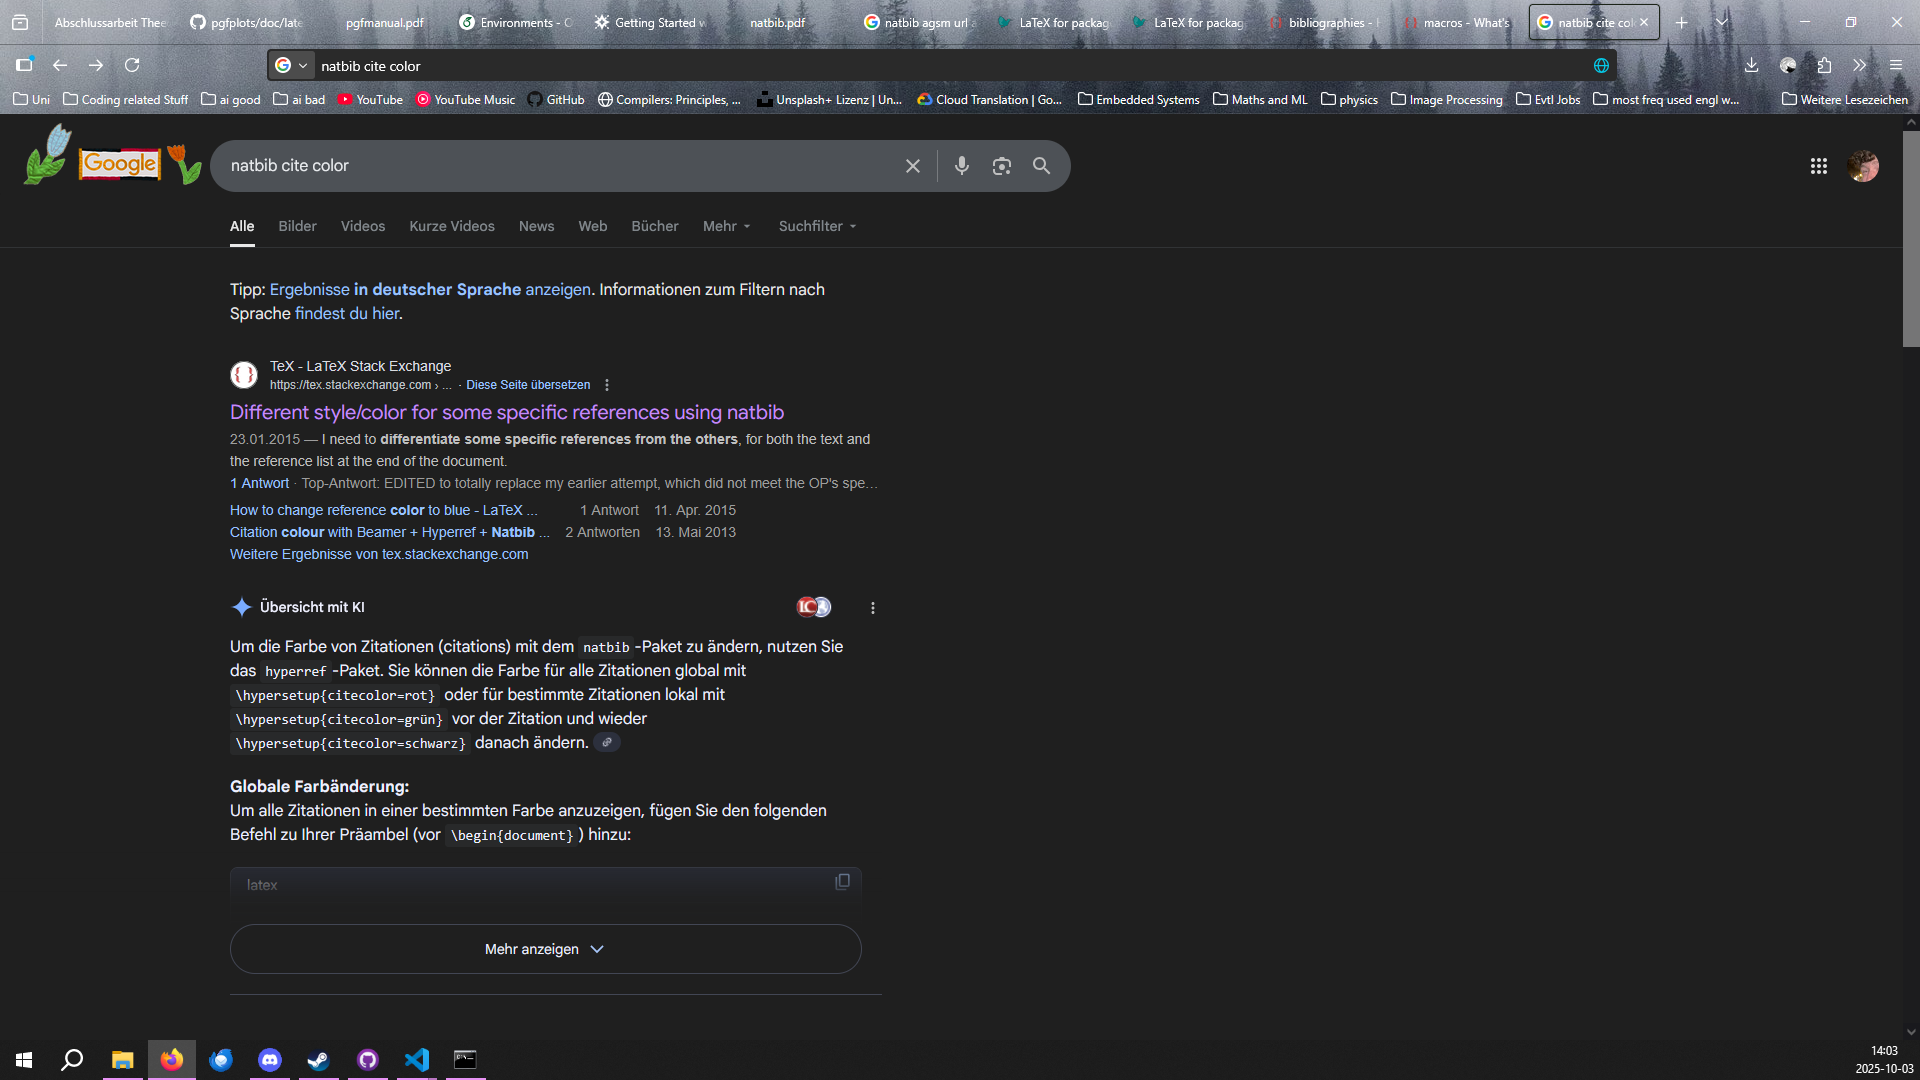
\includegraphics[width=\textwidth]{pictures/motivation.PNG}\label{fig:googlemakesmistakes}
\end{figure}
\endgroup

\end{document}